\tikzset{every picture/.style={line width=0.75pt}} %set default line width to 0.75pt        

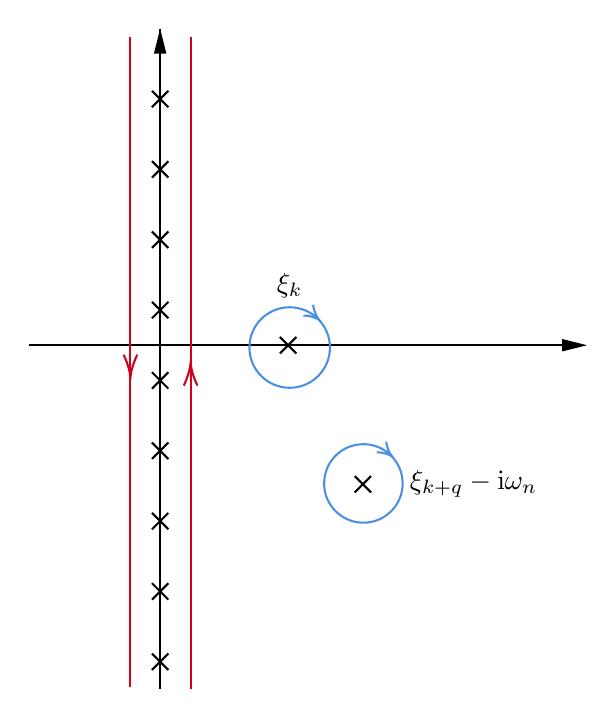
\begin{tikzpicture}[x=0.75pt,y=0.75pt,yscale=-1,xscale=1]
%uncomment if require: \path (0,379); %set diagram left start at 0, and has height of 379

%Straight Lines [id:da4696139814770115] 
\draw [color={rgb, 255:red, 208; green, 2; blue, 27 }  ,draw opacity=1 ]   (275,21.67) -- (275,334.67) ;
%Straight Lines [id:da08437675696747471] 
\draw    (226,170.17) -- (493,170.17) ;
\draw [shift={(495,170.17)}, rotate = 180] [fill={rgb, 255:red, 0; green, 0; blue, 0 }  ][line width=0.08]  [draw opacity=0] (12,-3) -- (0,0) -- (12,3) -- cycle    ;
%Straight Lines [id:da3198194636768519] 
\draw    (289.33,335.67) -- (289.33,19.67) ;
\draw [shift={(289.33,17.67)}, rotate = 450] [fill={rgb, 255:red, 0; green, 0; blue, 0 }  ][line width=0.08]  [draw opacity=0] (12,-3) -- (0,0) -- (12,3) -- cycle    ;
%Straight Lines [id:da33911829063354104] 
\draw    (289.33,17.67) -- (289.33,51.56) ;
\draw [shift={(289.33,51.56)}, rotate = 135] [color={rgb, 255:red, 0; green, 0; blue, 0 }  ][line width=0.75]    (-5.59,0) -- (5.59,0)(0,5.59) -- (0,-5.59)   ;
%Straight Lines [id:da9683910595635019] 
\draw    (289.33,51.56) -- (289.33,85.44) ;
\draw [shift={(289.33,85.44)}, rotate = 135] [color={rgb, 255:red, 0; green, 0; blue, 0 }  ][line width=0.75]    (-5.59,0) -- (5.59,0)(0,5.59) -- (0,-5.59)   ;
%Straight Lines [id:da23125512620723487] 
\draw    (289.33,85.44) -- (289.33,119.33) ;
\draw [shift={(289.33,119.33)}, rotate = 135] [color={rgb, 255:red, 0; green, 0; blue, 0 }  ][line width=0.75]    (-5.59,0) -- (5.59,0)(0,5.59) -- (0,-5.59)   ;
%Straight Lines [id:da9012438256404278] 
\draw    (289.33,119.33) -- (289.33,153.22) ;
\draw [shift={(289.33,153.22)}, rotate = 135] [color={rgb, 255:red, 0; green, 0; blue, 0 }  ][line width=0.75]    (-5.59,0) -- (5.59,0)(0,5.59) -- (0,-5.59)   ;
%Straight Lines [id:da9577216099300172] 
\draw    (289.33,153.22) -- (289.33,187.11) ;
\draw [shift={(289.33,187.11)}, rotate = 135] [color={rgb, 255:red, 0; green, 0; blue, 0 }  ][line width=0.75]    (-5.59,0) -- (5.59,0)(0,5.59) -- (0,-5.59)   ;
%Straight Lines [id:da12515690343677166] 
\draw    (289.33,187.11) -- (289.33,221) ;
\draw [shift={(289.33,221)}, rotate = 135] [color={rgb, 255:red, 0; green, 0; blue, 0 }  ][line width=0.75]    (-5.59,0) -- (5.59,0)(0,5.59) -- (0,-5.59)   ;
%Straight Lines [id:da5860572173856167] 
\draw    (289.33,221) -- (289.33,254.89) ;
\draw [shift={(289.33,254.89)}, rotate = 135] [color={rgb, 255:red, 0; green, 0; blue, 0 }  ][line width=0.75]    (-5.59,0) -- (5.59,0)(0,5.59) -- (0,-5.59)   ;
%Straight Lines [id:da2632609556473693] 
\draw    (289.33,254.89) -- (289.33,288.78) ;
\draw [shift={(289.33,288.78)}, rotate = 135] [color={rgb, 255:red, 0; green, 0; blue, 0 }  ][line width=0.75]    (-5.59,0) -- (5.59,0)(0,5.59) -- (0,-5.59)   ;
%Straight Lines [id:da5620983068494032] 
\draw    (289.33,288.78) -- (289.33,322.67) ;
\draw [shift={(289.33,322.67)}, rotate = 135] [color={rgb, 255:red, 0; green, 0; blue, 0 }  ][line width=0.75]    (-5.59,0) -- (5.59,0)(0,5.59) -- (0,-5.59)   ;
%Straight Lines [id:da21282805052989584] 
\draw    (230,170.17) -- (351,170.17) ;
\draw [shift={(351,170.17)}, rotate = 45] [color={rgb, 255:red, 0; green, 0; blue, 0 }  ][line width=0.75]    (-5.59,0) -- (5.59,0)(0,5.59) -- (0,-5.59)   ;
%Straight Lines [id:da0020189550089222408] 
\draw    (387,237.17) ;
\draw [shift={(387,237.17)}, rotate = 45] [color={rgb, 255:red, 0; green, 0; blue, 0 }  ][line width=0.75]    (-5.59,0) -- (5.59,0)(0,5.59) -- (0,-5.59)   ;
%Straight Lines [id:da27901434379198053] 
\draw [color={rgb, 255:red, 208; green, 2; blue, 27 }  ,draw opacity=1 ]   (304,335.67) -- (304,21.67) ;
\draw [shift={(304,178.67)}, rotate = 450] [color={rgb, 255:red, 208; green, 2; blue, 27 }  ,draw opacity=1 ][line width=0.75]    (10.93,-3.29) .. controls (6.95,-1.4) and (3.31,-0.3) .. (0,0) .. controls (3.31,0.3) and (6.95,1.4) .. (10.93,3.29)   ;
%Straight Lines [id:da7266322759719097] 
\draw [color={rgb, 255:red, 208; green, 2; blue, 27 }  ,draw opacity=1 ]   (275,36.67) -- (275,334.67) ;
\draw [shift={(275,185.67)}, rotate = 270] [color={rgb, 255:red, 208; green, 2; blue, 27 }  ,draw opacity=1 ][line width=0.75]    (10.93,-3.29) .. controls (6.95,-1.4) and (3.31,-0.3) .. (0,0) .. controls (3.31,0.3) and (6.95,1.4) .. (10.93,3.29)   ;
%Shape: Ellipse [id:dp2554624294784811] 
\draw  [color={rgb, 255:red, 74; green, 144; blue, 226 }  ,draw opacity=1 ] (332.33,171.27) .. controls (332.33,160.55) and (341.02,151.87) .. (351.73,151.87) .. controls (362.45,151.87) and (371.13,160.55) .. (371.13,171.27) .. controls (371.13,181.98) and (362.45,190.67) .. (351.73,190.67) .. controls (341.02,190.67) and (332.33,181.98) .. (332.33,171.27) -- cycle ;
\draw  [color={rgb, 255:red, 74; green, 144; blue, 226 }  ,draw opacity=1 ] (362.99,150.67) .. controls (363.43,153.65) and (364.39,156.05) .. (365.85,157.88) .. controls (363.87,156.62) and (361.38,155.95) .. (358.36,155.84) ;

%Shape: Ellipse [id:dp2358273364781196] 
\draw  [color={rgb, 255:red, 74; green, 144; blue, 226 }  ,draw opacity=1 ] (368.33,236.75) .. controls (368.33,226.3) and (376.8,217.84) .. (387.25,217.84) .. controls (397.7,217.84) and (406.16,226.3) .. (406.16,236.75) .. controls (406.16,247.2) and (397.7,255.67) .. (387.25,255.67) .. controls (376.8,255.67) and (368.33,247.2) .. (368.33,236.75) -- cycle ;
\draw  [color={rgb, 255:red, 74; green, 144; blue, 226 }  ,draw opacity=1 ] (398.23,216.67) .. controls (398.65,219.57) and (399.58,221.92) .. (401.02,223.7) .. controls (399.08,222.48) and (396.65,221.81) .. (393.71,221.71) ;


% Text Node
\draw (351.73,148.87) node [anchor=south] [inner sep=0.75pt]    {$\xi _{\boldsymbol{k}}$};
% Text Node
\draw (408.16,236.75) node [anchor=west] [inner sep=0.75pt]    {$\xi _{\boldsymbol{k} +\boldsymbol{q}} -\mathrm{i} \omega _{n}$};

\end{tikzpicture}